\documentclass[a4paper]{report}
\usepackage{graphicx}
\usepackage{ragged2e}
\usepackage{xcolor}
\usepackage[nottoc]{tocbibind}
\setcounter{secnumdepth}{3}
\setcounter{tocdepth}{3}
\usepackage{amssymb,amsmath,amsthm}
\pagestyle{empty}


\usepackage[style=authoryear,sorting=none]{biblatex}

\begin{document}
	
%	\begin{Robot Programming}
\tableofcontents
\newpage		
		
\section{Coordinate systems}
\subsection{Axis specific}

\subsection{Cartesian}
\subsubsection{Coordinate systems in conjunction with robots}
The following Cartesian coordinate systems are defined in the robot controller:
\begin{itemize}
	\item WORLD Coordinate System
	\newline
	Fixed, rectangular coordinate system whose origin is located at the base of the robot. It is the root coordinate system for the ROBROOT and BASE coordinate systems.
	By default, the WORLD coordinate system is located at the robot base.
	\item ROBROOT Coordinate System
	\newline
	Fixed, rectangular coordinate system whose origin is located at the base of the robot. It is the root coordinate system for the ROBROOT and BASE coordinate systems.
	By default, the WORLD coordinate system is located at the robot base.
	\item BASE Coordinate System
	Fixed, rectangular coordinate system whose origin is located at the base of the robot. It is the root coordinate system for the ROBROOT and BASE coordinate systems.
	By default, the WORLD coordinate system is located at the robot base.
	\item TOOL Coordinate System
	\newline
	a Cartesian coordinate system which is located at the tool center by default, the origin of the TOOL coordinate system is located at the flange center point. The TOOL coordinate system is offset to the tool center point by the user

\end{itemize}

\begin{figure}[h]
	\caption{KUKA robot coordinate systems}
	\centering
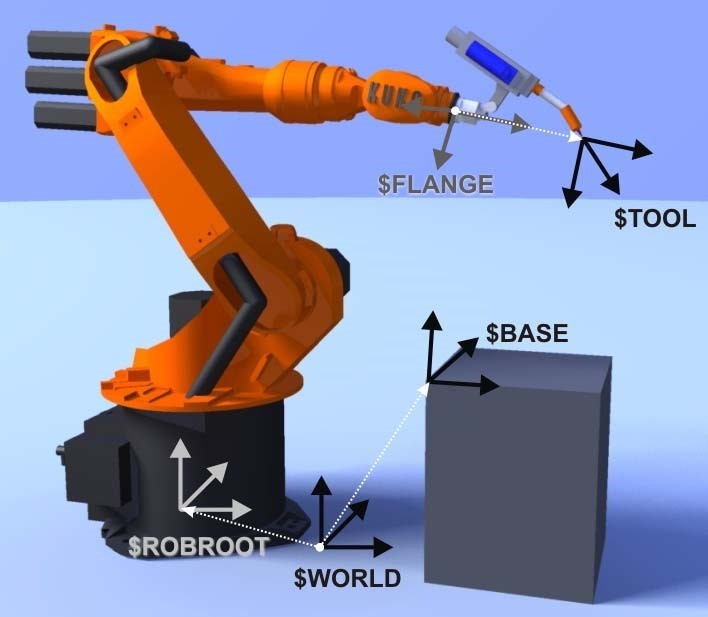
\includegraphics[scale=0.7]{kuka_coordinate_system.jpg}
\end{figure} 
\newpage
\section{KUKA Robot Language (KRL) Quick Guide}
KRC 4 controller uses KRL KUKA programming language.
\subsection{Variables and Declarations}
All system variables start with \textdollar sign, mind not starting any "user-defined" name with this sign to avoid syntax errors.
\vspace{0.5cm}
\subsubsection{Names in KRL}
\begin{itemize}
	\item Can have a maximum length of 24 characters
	\item Can consist of letters(A - Z), numbers(0 - 9) and the special characters '\textdollar'.
	\item Must not begin with a number.
	\item Must not be a keyword.
\end{itemize}
\subsubsection{Declaration and initialization of variables}
\begin{itemize}
	\item Variables (simple and complex) must be declared in the SRC file before the INI line and initialized after the INI line
	\item Variables can optionally also be declared and initialized in a local or global data list. 
	\item Every variable is linked to specific data type.
	\item The data type must be declared before use.
	\item The keyword for the declaration is DECL. It can be omitted in case of the four simple data type	
	\item In order to place syntax before the INI line, the DEF line must be activated:
	
	\centering	\textbf{  Open file \textgreater Edit \textgreater View \textgreater DEF line}
\end{itemize}

\fbox{\begin{minipage}{32em}
		
		DEF program name ( )
		\newline
		DECL data type user defined variable
		\newline;  declaration section of  variables
		\newline
		INI 
		\newline; Initialization section of user defined variables.
		\newline…
		\newline; Instruction Section
		\newline
		...
		\newline
		END
		
	\end{minipage}
	
}
\subsubsection{Simple Data types }
 
\begin{table}[h!]
	\centering
\begin{tabular}{| p{2cm} |p{3cm}|p{3cm}| p{2cm}| p{2cm}|}
	\hline
	\large Data Type & \large Integer & \large Real &\large Boolean &\large Character\\
	\hline
	\large Keyword & \large INT & \large REAL &\large BOOL &\large CHAR\\
	\hline
	\large Meaning & \large Floating point number & \large Logic state &\large Boolean &\large Character\\
	\hline
	\large Range & \large $-2^31 … 2^31-1$ & \large $±1.1E-38 … ±3.4E+38$ &\large TRUE, FALSE &\large ASCII character\\
	\hline
	\large Example & \large 2 & \large 4.23 &\large TRUE &\large C\\
	\hline

\end{tabular}
	\caption{is an example of KRL Data Types}
\label{table:1}
\end{table}
\newpage

\large {\textbf {Structure Types}}

\begin{itemize}

	\item AXIS: A1 to A6 are angle values (rotational axes) or translation values (translational axes)
		\vspace{.2cm}
		\newline
	\fbox{\begin{minipage}{32em}
			\centering
			{Axis: A1 .., A2 .., A3 .., A4, A5 .., A6 .. }
		\end{minipage}
	}
\vspace{.2cm}
	\item FRAME: X, Y, and Z are space coordinates, while A, B, and C are the orientation of the coordinate system.
		\vspace{.02cm}
	\newline

	\fbox{\begin{minipage}{32em}
			\centering
			{FRAME: X .., Y .., Z .., A .., B .., C .. }
		\end{minipage}
	}
\newline

\item POS and E6POS:  S (Status) and T (Turn) define axis positions unambiguously
\vspace{.2cm}
\newline
	\fbox{\begin{minipage}{32em}
		\centering
		{POS: X .., Y .., Z .., A .., B .., C .., S ..., T }
	\end{minipage}
	
}
\end{itemize}

\vspace{0.05cm}

	\section{Motion Programming}
\subsection{Motion Types}
The robot can move in various motion types. Paths are created according to the operation of each axis. Thus, the robot can be controlled to create either linear or circular path.
\subsubsection{Axis-specific motion}
	   The robot guides the TCP along the fastest path to the end point. The fastest path is generally not the shortest path and is thus not a straight line. The first motion in the program must be PTP as status and turns are only evaluated here.
	   The coordinates of the end point are absolute.
	   \paragraph{characteristics}
	   
	  
	   \begin{itemize}
	   	\item smooth motion
	   	\item Robot can move from start to end singularity free. As long as both the starting and ending points are in the working envelope, the robot will get to the end point without collision or sudden movement. 
	   	\item	Control is much simpler than continuous path control. 
	   \end{itemize}
   \begin{figure}[h]
   	\caption{PTP Motion}
   	\centering
   	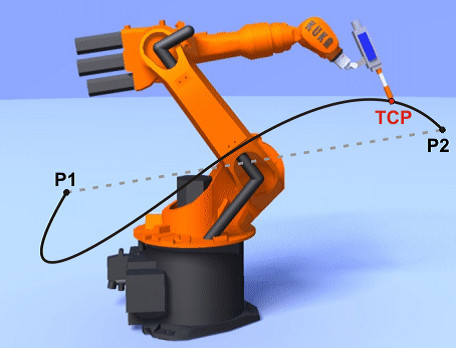
\includegraphics[scale=0.9]{ptp.png}
   \end{figure} 
	   
 \subsubsection{CP motion}
 \paragraph{LIN Motion}
 Motion at a defined velocity and acceleration along a straight line.  This motion requires the programmer to “teach” one point.  The robot uses the point defined in the previous move as the start point and the point defined in the current command as the end point and interpolates a straight line in between the two points.
 
 \begin{figure}[h]
 	\caption{LIN Motion}
 	\centering
 	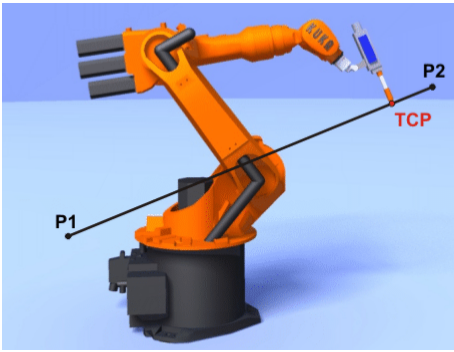
\includegraphics[scale=0.9]{LINmotion.png}
 \end{figure}
\paragraph{CIRC Motion}
Motion at a defined velocity and acceleration along a circular path or a portion of a circular path.  This motion requires the programmer to “teach” two points, the mid-point and the end point.  Using the start point of the robot (defined as the end point in the previous motion command) the robot interpolates a circular path through the mid-point and to the end point.
\begin{figure}[h]
	\centering
	\caption{CIRC Motion}
	\includegraphics[scale=0.9]{CIRCmotion.png}
\end{figure} 
\subsection{Approximate Positioning}
Approximate positioning of motion means that the next programmed point will not be exactly reached. This can help to shorten cycle times
 \begin{figure}[h]
	\caption{Speed Profile:
	\newline a) If all points approached exactly
	\newline b)In  case of approximate positioning of the points}
	\centering
	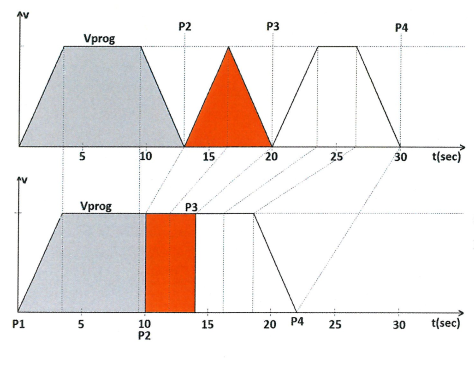
\includegraphics[scale=0.9]{approximateAdv.png}
\end{figure}
\begin{figure}[h]
	\caption{Approximate positioning of an auxiliary points}
	\centering
	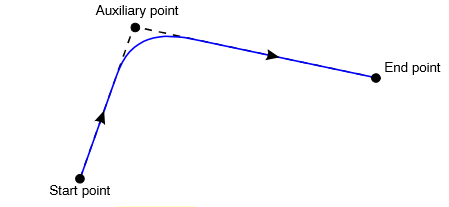
\includegraphics[scale=0.9]{apppos.png}
\end{figure}
\subsubsection{PTP-PTP approximate positioning }
For the purposes of PTP approximate positioning,the controller calculates the distances the axes are to move in the approximate positioning range, and plans velocity profiles for each axis which ensure tangential transition from the individual instructions to the approximate positioning contour.
\vspace{0.3cm} 
\newline System Variable, \textdollar APO.CPTP enables the start of approximate positioning to be specified as a percentage of these maximum values.
The approximate positioning of a point is displayed in the PTP command by adding the key word $C_PTP$: 


	\vspace{0.8cm} \centering \fbox{\begin{minipage}{32em}
		\centering
		\textdollar APO.CPTP = 80
		
		\vspace{0.1cm}
		PTP HOME $C_PTP$%



	\end{minipage}
}
	
\vspace{0.3cm} The greater this value the, the more path is rounded.
\newpage


\paragraph{Status and Turns}
\vspace{0.3cm}
The position of x,y,z and orientation A,B,C values of TCP are not sufficient to define the robot position ,as different axis positioning  are possible for the same TCP .
Status and turns serve to define the position that can be achieved with different axis positions.
\begin{figure}[h]
	\caption{Same TCP, different axis position}
	\centering
	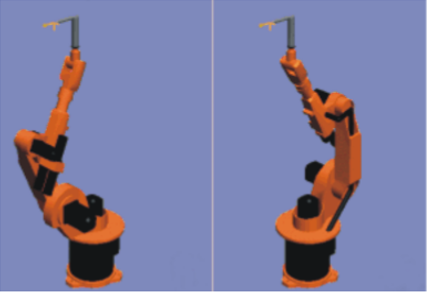
\includegraphics[scale=0.9]{ST.png}
\end{figure}
\subsection{User Programming}
Inline forms are available in the KSS for frequently used instruction. They simplify programming and facilitates user interface with controller without the need of knowing detail information about KUKA programming Language

 \subsection{Expert Programming}
 In the Expert interface, can achieve advanced programming using the KRL programming language and perform complex application programs including subprograms, interrupt programming, loops, and program branches. 
 

\clearpage
\end{document}